\documentclass[./\jobname.tex]{subfiles}
\begin{document}

\section{Problem Definition}
This chapter describes the broader idea of the \gls{wrm}, which is used to reformulate any differential equation into an optimisation problem and its application in the field of spectral methods (\cite{shen_spectral_2011}). The fitness function originates from these approaches. Further, the different approximation schemes and numerical solution representation are depicted. 

\subsection{Theoretical Foundation}
\label{chap:opt_problem}

The most general description of a linear \gls{pde} is displayed in equation \eqref{eq:general_pde}.
\begin{equation}
\label{eq:general_pde}
\begin{split}
\mathbf{L}u(\mathbf{x}) & = f(\mathbf{x}) \\
\text{subjected to: }\mathbf{B}u(\mathbf{x}) & = g(\mathbf{x}) \\
\end{split}
\end{equation}
This is similar to the formulation of the strong form in equation \eqref{eq: strong form}, but not limited to a Dirichlet boundary problem. The matrix $\mathbf{B}$ can include differentiation, effectively allowing i.e. Neumann boundary condition. 

An approximate solution to this problem is expressed as a finite sum of basis functions $\phi_k(\mathbf{x})$, as denoted in equation \eqref{eq:u_apx}. The coefficients $a_k$ need to be determined. In classical approximation schemes, the basis functions are orthogonal, such as trigonometric functions or Lagrange basis polynomials. 

\begin{equation}
\label{eq:u_apx}
u(\mathbf{x}) \approx u_{apx}(\mathbf{x}) = \sum_{k=0}^{N} a_k \phi_k (\mathbf{x})
\end{equation}

The residual of a \gls{pde}, as shown in equation \eqref{eq:residual}, is formulated as the difference between the left and the right side of the differential equation. The residual of a solved \gls{pde} is zero. This is only possible for the analytical solution, further denoted as $u_{ext}(x,y)$. For a numerical approximation $u_{apx}(x,y)$, the residual should be ''small enough``. 

\begin{equation}
\label{eq:residual}
R(\mathbf{x}) = \mathbf{L}u_{apx}(\mathbf{x}) - f(\mathbf{x})
\end{equation}

The \gls{wrm} (\cite{shen_spectral_2011}) tries to minimise this residual of a numerical candidate solution over the whole domain $\Omega$. Therefore, $R$ at every $\mathbf{x} \in \Omega$ is evaluated and added up, resulting in the following integral of equation \eqref{eq:wrm}. The residual at every $\mathbf{x}$ can be scaled by a weighting function over the domain as denoted with $W(\mathbf{x})$, which is needed for numerical stability and is linked to the Gauss Quadrature integration scheme. The choice of the test function $\psi(\mathbf{x})$ is distinct for different methods. The actual optimum does not change, since the zero-product property holds. The \gls{wrm} builds the basis for many solving strategies, including \gls{fem}. 

\begin{equation}
\label{eq:wrm}
WRF = \int_{\Omega} R(\mathbf{x}) \psi(\mathbf{x}) W(\mathbf{x}) dx
\end{equation}

This integral must be evaluated numerically. There are many different integration schemes available, but they are typically computational expensive. A less extensive approach is to evaluate the integral argument at different ``collocation points''. This can be seen in equation \eqref{eq:wrm_colloc}. Although it is not an integral per se, it does assign a numerical ``score'' to the residual. 

\begin{equation}
\label{eq:wrm_colloc}
\sum_{k=0}^{N} R(\mathbf{x}_k) \psi(\mathbf{x}_k) W(\mathbf{x}_k)
\end{equation}

To ensure that negative and positive residuals do not cancel each other out, a common choice in heuristic methods from table \ref{tab:results_literature_comparison} is to choose $\psi(\mathbf{x}_k)$ as the residual itself, effectively squaring it. The resulting ``sum of squared residuals'' forms the basis for nearly all fitness functions in the current literature, as represented in equation \eqref{eq:sum_squared_residual}.

\begin{equation}
\label{eq:sum_squared_residual}
\sum_{k=0}^{N} R(\mathbf{x}_k)^2 W(\mathbf{x}_k)
\end{equation}

These methods are often called ``spectral methods'' (\cite{shen_spectral_2011}). Their main advantage over finite difference methods is that they take the whole domain into account. The derivative of the function at one point is influenced by the function at every other point in the domain. This global approach can lead to a better accuracy. 

\subsection{Fitness Function}
\label{chap:fit_func}

As mentioned above, the basis of the fitness function used in \cite{chaquet_using_2019} is the squared weighted residual in equation \eqref{eq:sum_squared_residual}. They split the summation over the collocation points into two parts: the points on the boundary ($n_B$) and the points on the inner domain ($n_C$). Further, they divide the fitness value by the number of points used. This fitness function, as seen in equation \eqref{eq:fit_func_chaquet}, is adopted in this thesis. Because here, systems of differential equations are not considered, the denominator changes to $m=1$ resulting in the fitness function \eqref{eq:fit_func} below. The norm around the residual is not necessary for this thesis, since the fitness function does not have to work for System of \gls{pde}s.

\begin{equation}
\label{eq:fit_func}
F(u_{apx}(\mathbf{x})) = \frac{\sum_{i=1}^{n_C} \xi (\mathbf{x}_i) \left[ \mathbf{L}u_{apx}(\mathbf{x}_i) - f(\mathbf{x}_i) \right]^2 + \phi \sum_{j=1}^{n_B} \left[ \mathbf{B}u_{apx}(\mathbf{x}_j) - g(\mathbf{x}_j)\right]^2}{(n_C + n_B)}  
\end{equation}

A notable property of the fitness function is that it can not drop below 0. A solution, that satisfies the residual at every $n_C$ and $n_B$, results in a fitness of 0. This is true for the analytical solution $u_{apx}(\mathbf{x})$. It is also important to notice, that aliasing errors (as described in the chapter \ref{chap:metric_quality}) can occur with this fitness function. 

The weighting function is also split into two parts: $\xi$ for the inner collocation points and $\phi$ as penalty factor for the boundary points. The weighting function $\xi$ can be adapted by a parameter $\kappa$. For a $\kappa > 0$, $\xi$ assigns larger values for collocation points closer to the boundary, effectively shifting the relative importance towards the boundary. These weights can be calculated a priori, so no computational effort is added to the fitness function. Again, the weights are directly extracted from \cite{chaquet_using_2019}. 

\begin{equation}
\label{eq:nc_weight}
\xi(\mathbf{x}_i) = \frac{1 + \kappa \left(1 - \frac{min_{\forall \mathbf{x}_j\in n_B}|| \mathbf{x}_i - \mathbf{x}_j ||}{max_{\forall\mathbf{x}_k \in n_C}(min_{\forall \mathbf{x}_j \in n_B} || \mathbf{x}_k - \mathbf{x}_j ||)}\right)}{1 + \kappa}
\end{equation}


\subsection{Candidate Representation}
\label{chap:candidate_rep}

As \cite{chaquet_using_2019} suggest, an approximate solution should be represented as a summation of $N$ scaled and shifted radial basis functions $\phi$, as stated in equation \eqref{eq:u_apx} Gauss kernels have frequently been used for the approximation of functions. A solid foundation on the approximation theorem can be seen in \cite{park_universal_1991}. \gls{rbf} are functions that are point symmetric to a centre $c$ and their function value only depends on the radius $r$. 

\begin{equation}
\label{eq: radius}
r = \left|\left|\mathbf{x} - \mathbf{c} \right|\right|
\end{equation}

This thesis mainly works with two different types of \gls{rbf}. The first one is the classical Gauss \gls{rbf} ($gak$). The second one, further called GSin \gls{rbf} ($gsk$), is more complex. A candidate solution is represented as the parameters that shift and deform these \gls{rbf}. 

\subsubsection{Gauss Kernel}
\label{chap:gauss_kernel}

In general, a \gls{gak} is the classical choice to approximate functions. It was first introduced in \cite{broomhead_multivariable_1988}. Equation \eqref{eq:gauss_kernel} shows the formulation of such a kernel. One kernel has 4 parameters, that change its shape and location. $\omega$ is a scaling factor for each and $\gamma$ describes how sharp the e-function is. Depending on the space the solution is defined in, the number of values in the vector $\mathbf{c}$ could change - one for each dimension. However, in this work only $\mathbb{R}^2$ is of interest, thus $\mathbf{c}$ always includes 2 values. In figure \ref{fig:gauss_kernel_3d_plot} a single standard \gls{gak} is plotted. 

\begin{equation}
\label{eq:gauss_kernel}
gak(\mathbf{x}) = \omega e^{-\gamma ||\mathbf{x} - \mathbf{c}||^2}
\end{equation}

\begin{figure}[H]
	\centering
	\noindent\adjustbox{max width=\linewidth}{
		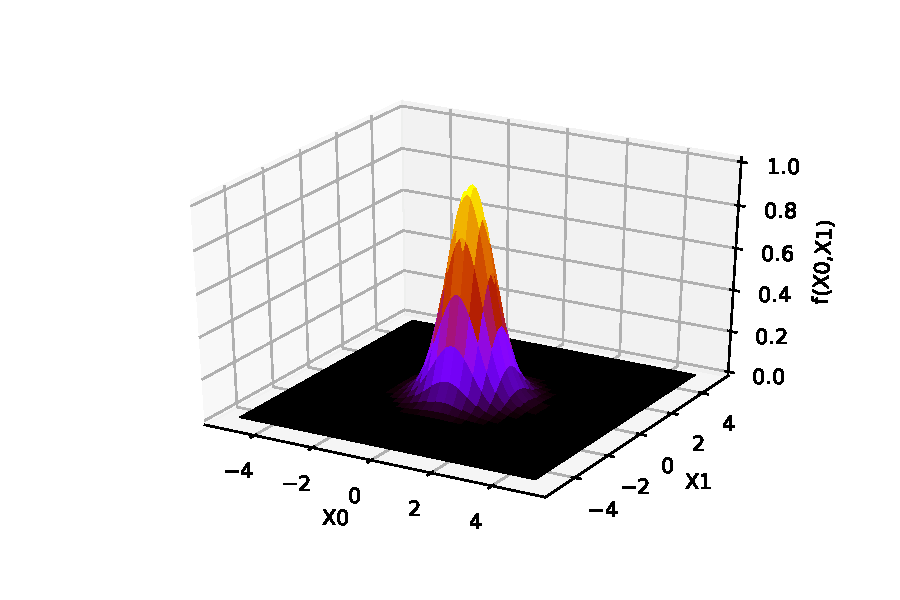
\includegraphics[width=\textwidth]{../../code/kernels/gak.pdf}
	}
	\unterschrift{3D plot of a single Gauss kernel with the parameters $\omega = 1$, $\gamma = 1$, $c_0 = 0$ and $c_1 = 0$}{}{}
	\label{fig:gauss_kernel_3d_plot}
\end{figure}

An approximate solution to the \gls{pde} in question is described as the superposition of $N$ kernels as shown in equation \eqref{eq:uapx_gauss_kernel}. 

\begin{equation}
\label{eq:uapx_gauss_kernel}
u_{apx}(\mathbf{x}) = \sum_{i=0}^{N} \omega_i e^{-\gamma_i r_i^2}
\end{equation}

A solution is encoded as a vector of these $4\cdot N$ parameters stacked together. This is shown in equation \eqref{eq:gauss_parameter_vector}. 

\begin{equation}
\label{eq:gauss_parameter_vector}
\mathbf{p_{apx}} = \left[\underbrace{\omega_0, \gamma_0, c_{00}, c_{01}}_{\text{kernel 0}}, \cdots \underbrace{\omega_i, \gamma_i, c_{i0}, c_{i1}}_{\text{kernel i}}, \cdots \underbrace{\omega_N, \gamma_N, c_{N0}, c_{N1}}_{\text{kernel N}} \right]^T
\end{equation}

To evaluate the residual of a \gls{pde}, the derivatives must be known. To that extend, the derivative of $u_{apx}$ from equation \eqref{eq:u_apx} is calculated. The first order derivative with respect to $x_0$ is seen in equation \eqref{eq:uapx_gauss_kernel_x0}. To solve the proposed testbed, also the second order derivatives are needed, as described in equation \eqref{eq:uapx_gauss_kernel_x0x0}. Although the mixed term derivative is not used in this work, for the sake of completeness it is displayed in equation \eqref{eq:uapx_gauss_kernel_x0x1}.  


\begin{equation}
\label{eq:uapx_gauss_kernel_x0}
\frac{\partial u_{apx}(\mathbf{x})}{\partial x_j} = -2 \sum_{i=0}^{N} \omega_i \gamma_i (x_j - c_{ij}) e^{-\gamma_i r_i^2}
\end{equation}

\begin{equation}
\label{eq:uapx_gauss_kernel_x0x0}
\frac{\partial^2 u_{apx}(\mathbf{x})}{\partial x_j^2} = \sum_{i=0}^{N} \omega_i \gamma_i \left[ 4 \gamma_i (x_j - c_{ij})^2 - 2 \right] e^{-\gamma_i r_i^2}
\end{equation}

\begin{equation}
\label{eq:uapx_gauss_kernel_x0x1}
\frac{\partial^2 u_{apx}(\mathbf{x})}{\partial x_j x_k} = 4 \sum_{i=0}^{N} \omega_i \gamma_i^2 (x_j - c_{ij}) (x_k - c_{ik}) e^{-\gamma_i r_i^2} 
\end{equation}

\subsubsection{GSin Kernel}
\label{chap:gsin_kernel}
Additional to the Gauss kernel, a ``GSin'' kernel, further also abbreviated as \gls{gsk}, is proposed. In essence, this is a multiplication of a \gls{gak} with a sine function, as seen in equation \eqref{eq:gsin_kernel}. It can be thought of a sine function, where its influence declines with the radius $r$. The plot in figure \ref{fig:gsin_kernel_3d_plot} shows how the first half period is much larger than the second half. Both ``sub-functions'' are centred at the same $\mathbf{c}$. As shown in chapter \ref{chap:gsin_approximation_theorem}, the universal approximation theorem for the GSin kernel holds true. 
With the sine, two new parameters are introduced: $f$ for the frequency of the sine wave and $\varphi$ represents the phase shift. 
\begin{equation}
\label{eq:gsin_kernel}
gsk(\mathbf{x}) = \omega e^{-\gamma ||\mathbf{x} - \mathbf{c}||^2} sin(f ||\mathbf{x} - \mathbf{c}||^2 - \varphi)
\end{equation}

It is important to notice that, with the correct parameter choice, both traits - the sine and the e-function - can be retrieved. When $\gamma=0$ the e-function evaluates to 1 and leaves the sine on its own. By setting $f=0$ and $\varphi=-\frac{\pi}{2}$, the sine resolves to 1 and the e-function part is obtained. Thus, with this kernel it should be possible to approximate more functions than the \gls{gak}. 

\begin{figure}[H]
	\centering
	\noindent\adjustbox{max width=\linewidth}{
		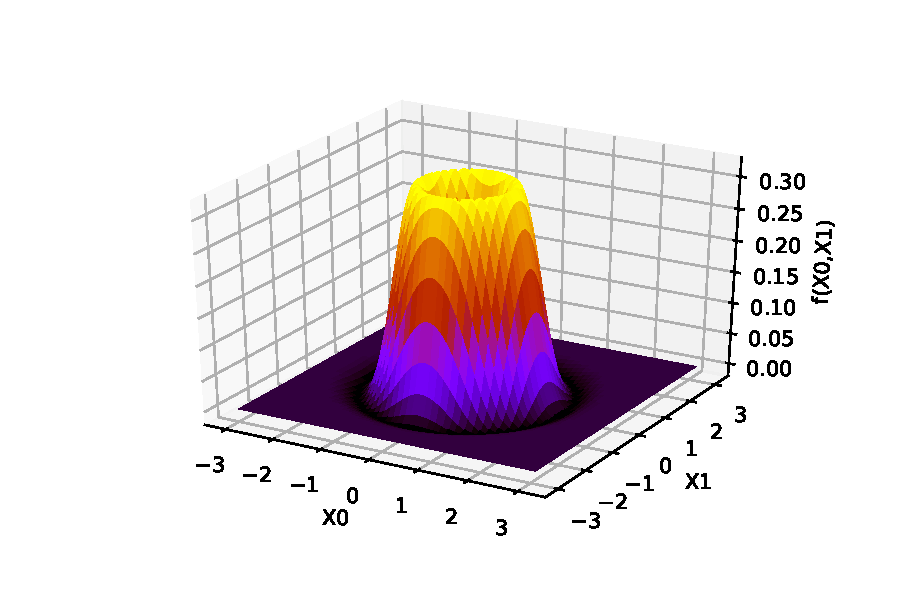
\includegraphics[width=\textwidth]{../../code/kernels/gsk.pdf}
	}
	\unterschrift{3D plot of a single GSin kernel with the parameters $\omega = 1$, $\gamma = 1$, $c_0 = 0$, $c_1 = 0$, $f = 1$, $\varphi = 0$}{}{}
	\label{fig:gsin_kernel_3d_plot}
\end{figure}

Similar to the Gauss kernel, the approximate solution is described as the superposition of $N$ GSin kernels, as seen in equation \eqref{eq:uapx_gsin_kernel}. 

\begin{equation}
\label{eq:uapx_gsin_kernel}
u_{apx}(\mathbf{x}) = \sum_{i=0}^{N} \omega_i e^{\gamma_i r_i^2} sin(f_i r_i^2 - \varphi_i)
\end{equation}

Equation \eqref{eq:gsin_parameter_vector} shows the solution representation in stacked vector notation, including the two new parameters $f$ and $\varphi$. 

\begin{equation}
\label{eq:gsin_parameter_vector}
\mathbf{p_{apx}} = \left[\underbrace{\omega_0, \gamma_0, c_{00}, c_{01}, f_0, \varphi_0}_{\text{kernel 0}}, \cdots \underbrace{\omega_i, \gamma_i, c_{i0}, c_{i1}, f_i, \varphi_i}_{\text{kernel i}}, \cdots \underbrace{\omega_N, \gamma_N, c_{N0}, c_{N1}, f_N, \varphi_N}_{\text{kernel N}} \right]^T
\end{equation}

Again, the derivatives of the solution are needed, which are shown in the equations \eqref{eq:uapx_gsin_kernel_x0} through \eqref{eq:uapx_gsin_kernel_x0_x1}. 

\begin{equation}
\label{eq:uapx_gsin_kernel_x0}
\frac{\partial u_{apx}(\mathbf{x})}{\partial x_j} = \sum_{i=0}^{N} 2 \omega_i (x_j - c_{ij}) e^{-\gamma_i r_i^2} (f_i cos(f_i r_i^2 - \varphi_i)-\gamma_i sin(f_i r_i^2 - \varphi_i))
\end{equation}

\begin{equation}
\label{eq:uapx_gsin_kernel_x0_x0}
\begin{split}
\frac{\partial^2 u_{apx}(\mathbf{x})}{\partial x_j^2} = & \sum_{i=0}^{N} 2 \omega_i e^{-\gamma_i r_i^2} \\ [  -(2(f_i^2 - \gamma_i^2) (x_j-c_{ij})^2 + \gamma_i) sin(f_i r_i^2 - \varphi_i) - & (4 f_i \gamma_i (x_j-c_{ij})^2 -f_i) cos(f_i r_i^2 - \varphi_i) ] 
\end{split}
\end{equation}

\begin{equation}
\label{eq:uapx_gsin_kernel_x0_x1}
\begin{split}
& \frac{\partial^2 u_{apx}(\mathbf{x})}{\partial x_j x_k} = \sum_{i=0}^{N} -4 \omega_i (c_{ij} - x_j) (c_{ik} - x_k) e^{-\gamma_i r_i^2} \\ & \left[(f_i^2 - \gamma_i^2) sin(f_i r_i^2 - \varphi_i) + 2 f_i \gamma_i cos(f_i r_i^2 - \varphi_i)\right]
\end{split}
\end{equation}

\end{document}